\documentclass[11pt]{article}
\usepackage[margin=0.75in]{geometry}
\usepackage[T1]{fontenc}
\usepackage{lmodern}
\usepackage{xcolor}
\usepackage{graphicx}
\usepackage{booktabs}
\usepackage{array}
\usepackage{tabularx}
\usepackage{enumitem}
\usepackage{hyperref}
\usepackage{xurl}
\usepackage{fancyvrb}

\hypersetup{colorlinks=true,linkcolor=blue,urlcolor=blue}
\setlength{\parindent}{0pt}
\setlength{\parskip}{5pt}
\setlist[itemize]{topsep=3pt,itemsep=2pt}
\newcolumntype{Y}{>{\raggedright\arraybackslash}X}

\begin{document}

\begin{center}
  {\LARGE\bfseries MCG 5353 Robotics Project 2}\\[3pt]
  {\large Panda Gazebo Color Sorting}
\end{center}

\textbf{Weight:} 15\% of course grade\\
\textbf{Platform:} ROS 2 Humble, Gazebo Classic, MoveIt 2, Panda arm\\
\textbf{Submission:} complete ROS 2 package + README + short demonstration video

\section*{Goal}

Create a ROS 2 Python package that commands the Panda robot to sort six
objects in Gazebo:

\begin{itemize}
  \item Move the three red boxes to the red container.
  \item Move the three blue boxes to the blue container.
  \item Use meaningful arm and gripper commands so the robot visibly performs
        the task.
  \item Leave the provided base package unchanged. Build your project package
        around it.
\end{itemize}

\begin{center}
  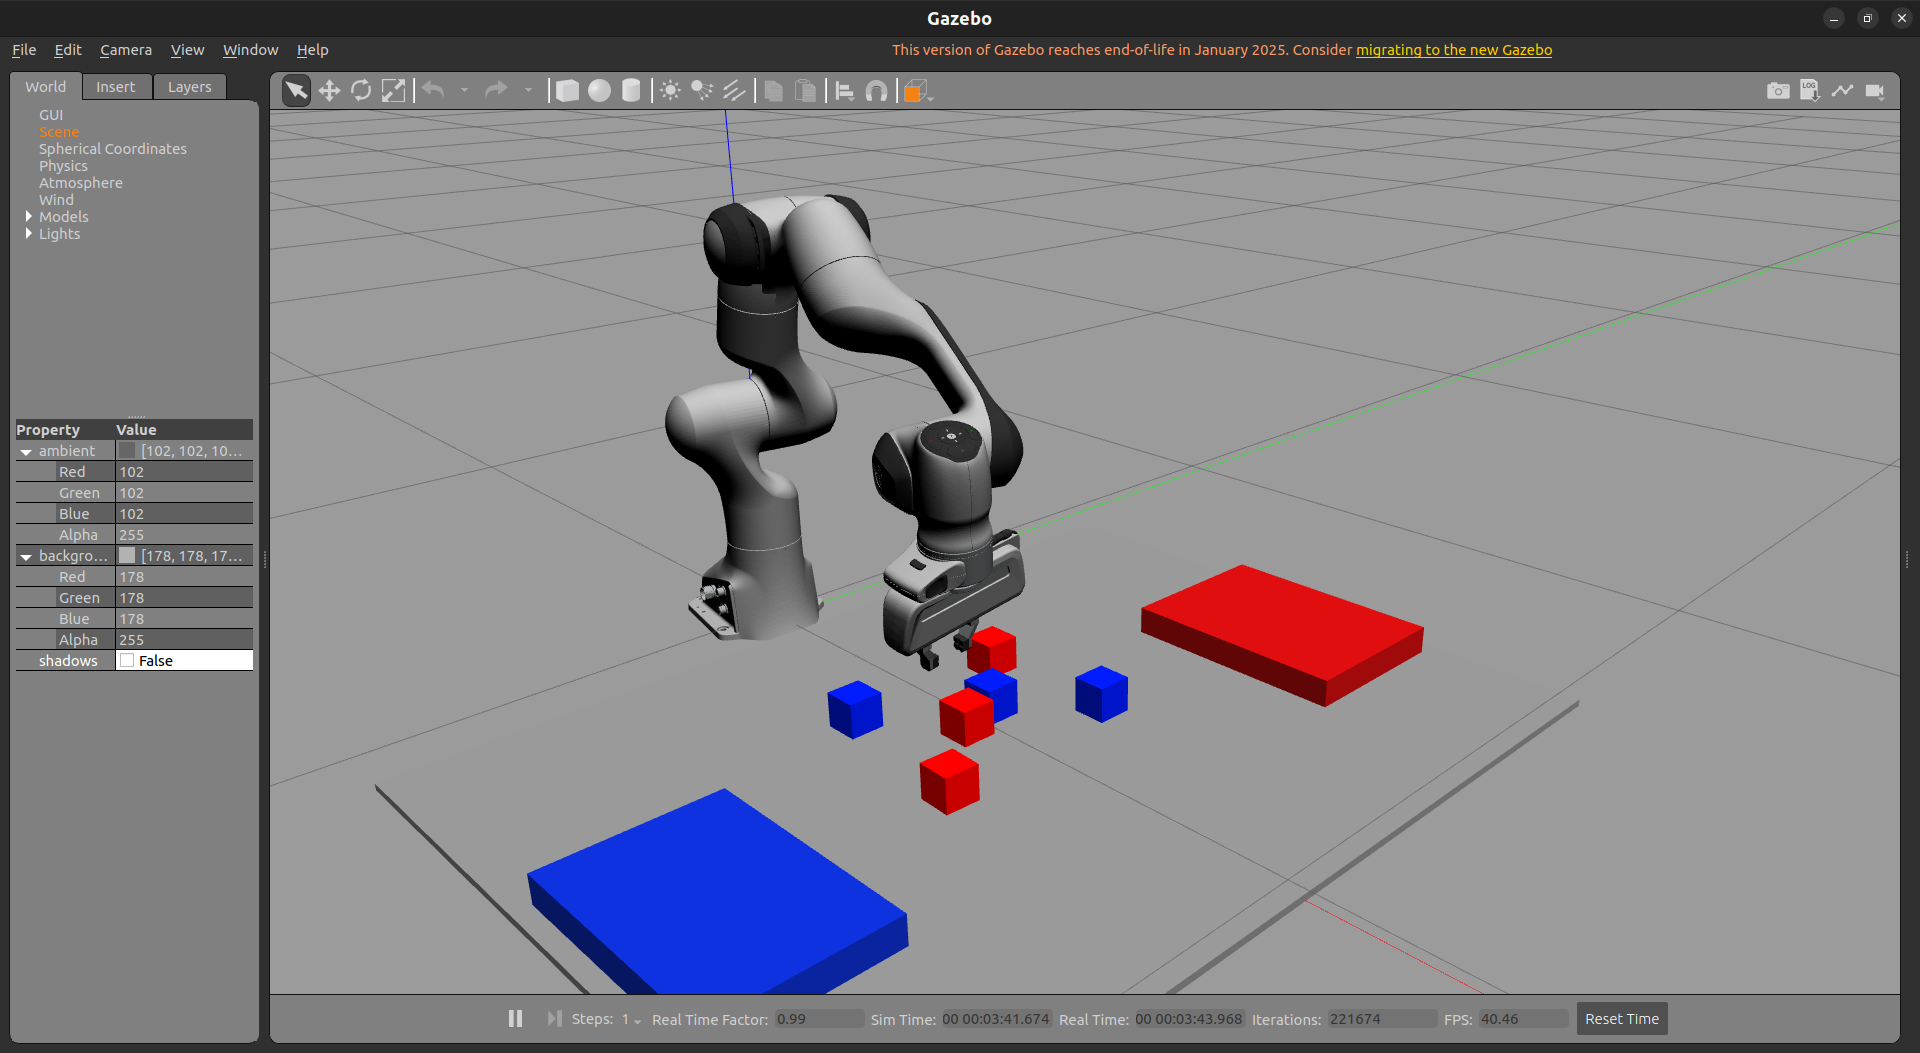
\includegraphics[width=0.92\textwidth]{panda_gazebo_color_sorting_task.png}

  \small Expected scene: mixed red and blue objects with matching destination containers.
\end{center}

\section*{Get The Base Package}

\begin{Verbatim}[fontsize=\small]
cd ~/ros2_ws/src
git clone https://github.com/ake1999/
mcg5353_panda_gazebo_moveit_pick_place_projects.git

cd ~/ros2_ws
colcon build --symlink-install \
  --packages-select mcg5353_panda_gazebo_moveit
source install/setup.bash
\end{Verbatim}

Run the prepared Panda Gazebo + MoveIt stack:

\begin{Verbatim}[fontsize=\small]
ros2 launch mcg5353_panda_gazebo_moveit \
  panda_moveit_gazebo.launch.py
\end{Verbatim}

Before writing your project logic, confirm that Panda remains upright, RViz
opens, MoveIt is ready, and all three controllers are active.

\section*{Create Your Project Package}

Create a separate package. You may choose a different valid package name.

\begin{Verbatim}[fontsize=\small]
cd ~/ros2_ws/src
ros2 pkg create --build-type ament_python \
  mcg5353_panda_sorting_project \
  --dependencies rclpy control_msgs trajectory_msgs \
  sensor_msgs geometry_msgs moveit_msgs
\end{Verbatim}

Your package should include:

\begin{itemize}
  \item \texttt{package.xml}, \texttt{setup.py}, and \texttt{setup.cfg};
  \item a Python node such as \texttt{sorting\_node.py};
  \item a console-script entry point so the node runs with \texttt{ros2 run};
  \item a README containing exact build, launch, and run commands.
\end{itemize}

\section*{Required Task}

The objects are named:

\begin{center}
\texttt{red\_box\_1}, \texttt{red\_box\_2}, \texttt{red\_box\_3},
\texttt{blue\_box\_1}, \texttt{blue\_box\_2}, \texttt{blue\_box\_3}.
\end{center}

The destinations are \texttt{red\_container} and \texttt{blue\_container}.

For each box, your task sequence should clearly include:

\begin{enumerate}[leftmargin=2em]
  \item move to a safe approach pose;
  \item open the gripper;
  \item approach the selected box;
  \item close the gripper or clearly apply your grasp/attachment logic;
  \item move toward the matching container;
  \item release the box;
  \item retreat to a safe pose.
\end{enumerate}

Develop incrementally: make one object work, then generalize the sequence to
all six objects. You may use MoveIt pose goals, controller joint goals, or a
well-explained combination.

\section*{Useful Interfaces}

\begin{tabularx}{\textwidth}{@{}p{0.39\textwidth}Y@{}}
\toprule
\textbf{Interface} & \textbf{Purpose} \\
\midrule
\texttt{/move\_action} & Ask MoveIt to plan and move toward a new robot pose. \\
\texttt{/panda\_arm\_controller/}\newline
\texttt{follow\_joint\_trajectory} & Execute known arm joint trajectories. \\
\texttt{/panda\_hand\_controller/}\newline
\texttt{gripper\_cmd} & Open or close the Panda gripper. \\
\texttt{/joint\_states} & Read current joint positions and velocities. \\
\texttt{gz model -m <name> -p} & Inspect a Gazebo model pose while debugging. \\
\bottomrule
\end{tabularx}

\section*{Required Demonstration}

Your video must show:

\begin{enumerate}[leftmargin=2em]
  \item the command used to launch the base package;
  \item Panda, both containers, and all six mixed-color boxes in Gazebo;
  \item your node started with \texttt{ros2 run};
  \item visible arm and gripper motion;
  \item all red boxes in the red container;
  \item all blue boxes in the blue container;
  \item one debug check, such as \texttt{ros2 control list\_controllers}.
\end{enumerate}

\section*{Grading: 100 Project Points}

Your score out of 100 is converted to the 15\% course weight.

\begin{tabularx}{\textwidth}{@{}Y>{\raggedleft\arraybackslash}p{0.13\textwidth}@{}}
\toprule
\textbf{Criterion} & \textbf{Points} \\
\midrule
Package builds, installs, and runs using documented commands & 10 \\
Correct integration with the provided Gazebo + MoveIt base package & 15 \\
Arm and gripper commands are used meaningfully and safely & 20 \\
All three red boxes reach the red container & 15 \\
All three blue boxes reach the blue container & 15 \\
Sequence is repeatable and handles all six objects clearly & 10 \\
Code organization, names, comments, and readable task logic & 5 \\
README and complete video evidence & 10 \\
\midrule
\textbf{Total} & \textbf{100} \\
\bottomrule
\end{tabularx}

\section*{Optional Computer-Vision Bonus: Up To +5 Project Points}

This is an advanced, optional extension. The bonus applies only to the
combined project component of the course (Project 1 + Project 2, worth 25\%).
It does not add marks to theory, exams, or other course components.

For the bonus, add a simulated camera and use image data to decide whether an
object is red or blue before choosing its destination. A reasonable approach
is:

\begin{itemize}
  \item add an RGB camera sensor and publish an image topic;
  \item subscribe to the image in your Python node;
  \item use a simple color-space threshold or segmentation method;
  \item connect the detected color to your sorting decision;
  \item show the camera image, detection result, and correct placement in the video.
\end{itemize}

The bonus requires working computer-vision evidence and an explanation in the
README. Merely adding a camera model is not enough. The maximum bonus is five
percentage points on the Project 2 score, capped according to course policy.

\section*{Submission Checklist}

\begin{itemize}
  \item Complete Project 2 ROS 2 package;
  \item no unfinished \texttt{NotImplementedError};
  \item README with build, launch, run, and dependency instructions;
  \item short video proving the required result;
  \item optional computer-vision files and explanation, if attempted.
\end{itemize}

\end{document}
